% document's head

\begin{center}
    \LARGE \textsc{Задание по квантовой механике I}
\end{center}

\hrule

\phantom{42}

\begin{flushright}
    \begin{tabular}{rr}
    % written by:
        % \textbf{Источник}: 
        % & \href{__ссылка__}{__название__} \\
        % & \\
        % \textbf{Лектор}: 
        % & _ФИО_ \\
        % & \\
        \textbf{Автор заметок}: 
        % \textbf{Авторы заметок}: 
        & Хоружий Кирилл \\
        % & Примак Евгений \\
        % & Гурьева Соня \\
        & \\
    % date:
        \textbf{От}: &
        \textit{\today}\\
    \end{tabular}
\end{flushright}

\thispagestyle{empty}
\tableofcontents

\vspace*{\fill}
\begin{figure}[h]
    \centering
    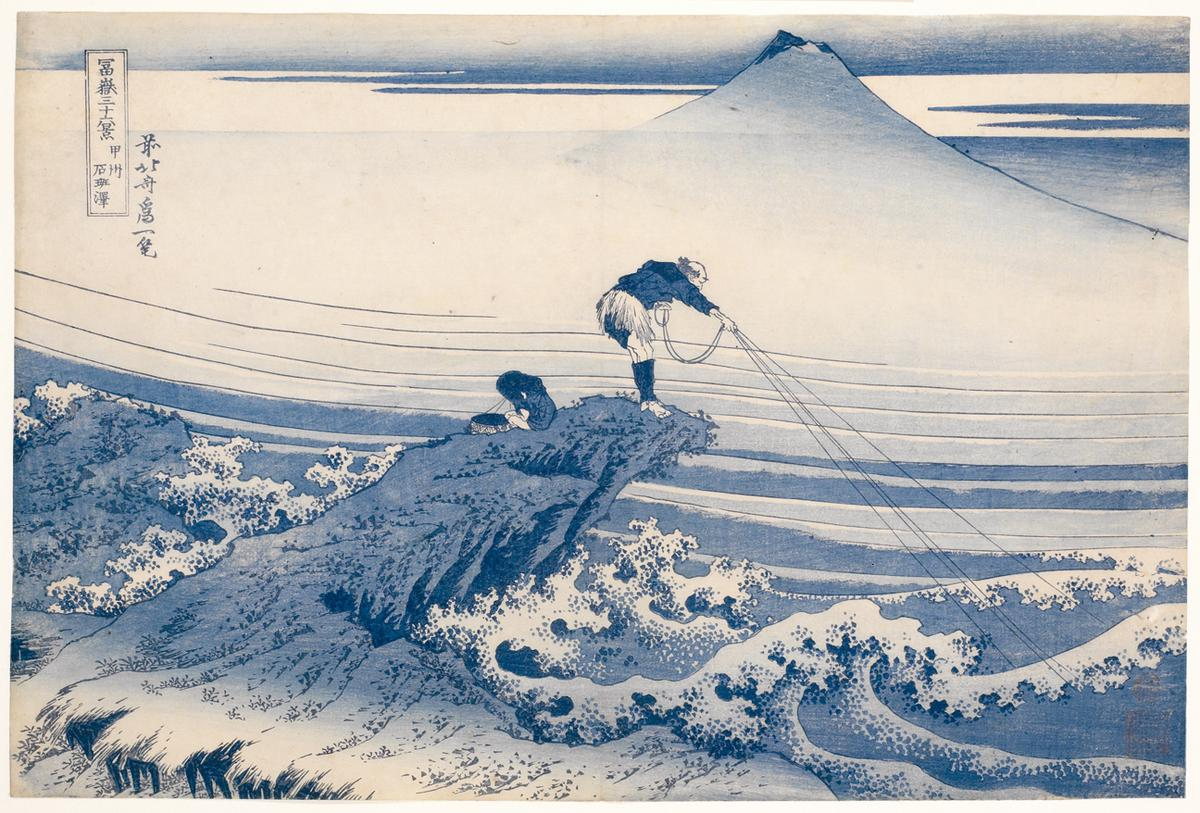
\includegraphics[width=0.95\textwidth]{figures/pic1.jpeg}
    %\caption{}
    %\label{fig:}
\end{figure}

\begin{flushright}
    \textcolor{gray}{
    \small{Также выражаем благодарность Мещрякову Павлу за консультации по отдельным задачам.}}
\end{flushright}
\newpage
